\documentclass{beamer}


\usepackage[utf8]{inputenc}
\usepackage{amsmath}
\usepackage{amsfonts}
\usepackage{amssymb}
\usepackage{graphicx}
\usepackage{ragged2e}  % `\justifying` text
\usepackage{booktabs}  % Tables
\usepackage{tabularx}
\usepackage{tikz}      % Diagrams
\usetikzlibrary{calc, shapes, backgrounds}
\usepackage{amsmath}
\usepackage{amssymb}
\usepackage{dsfont}
\usepackage{url}       % `\url
\usepackage{listings}  % Code listings
\usepackage[T1]{fontenc}


\usepackage{theme/beamerthemehbrs}
%\usepackage{preamble}


\author[Alex Mitrevski]{Alex Mitrevski}
\title{Introduction to Programming}
\subtitle{}
%\logo{}
\institute[HBRS]{Hochschule Bonn-Rhein-Sieg}
\date{March 20, 2018}
\subject{Introduction to Programming}

\begin{document}
{
\begin{frame}
\titlepage
\end{frame}
}

\AtBeginSection[]{% Print an outline at the beginning of sections
\begin{frame}<beamer>
    % \frametitle{Outline for Section \thesection}
    \tableofcontents[currentsection]
\end{frame}%
}%

\section{What is Programming?}

\begin{frame}{What is Programming?}
    Loosely speaking, programming means "giving detailed instructions to a computer about the way it should behave"
    \newline

    Detailed instructions because the computer is just a machine
    \newline

    On their own, computers have no intelligence, so we have to tell them what to do
\end{frame}

\section{Building Blocks of a Computer Program}

\begin{frame}
\frametitle{Algorithm}
    An algorithm is \emph{a set of \textbf{detailed} instructions that tell a computer how to behave}
    \newline

    Example algorithm: going to the supermarket
    \begin{enumerate}
        \item Take pen and paper
        \item Make a list of things to buy
        \item Leave the pen on the table
        \item Put the paper in the pocket
        \item Go out of the door
        \item ...
    \end{enumerate}
\end{frame}

\begin{frame}
\frametitle{Program}
    A program is a set of algorithms synchronized in a way that solves a specific problem
    \newline

    Example program: go to the supermarket
    \begin{enumerate}
        \item Execute algorithm \emph{Prepare}
        \item Execute algorithm \emph{Drive to the market}
        \item Execute algorithm \emph{Shop in the market}
        \item Execute algorithm \emph{Go back home}
    \end{enumerate}
\end{frame}

\begin{frame}
\frametitle{Computer Instructions}
    In everyday life, an instruction can be thought of as a recommendation (or a rule) for doing something in a certain way
    \newline

    In programming, instructions represent:
    \begin{itemize}
        \item Saving values in memory
        \item Retrieving values from memory
        \item Performing operations on the values stored in memory
    \end{itemize}
\end{frame}

\begin{frame}
\frametitle{Performing Instructions (2/2)}
    Most of the time, we programmers work with \emph{computer memory}
    \newline

    A useful analogy for memory is to model it by boxes and blocks (I owe this very useful model to my first programming professor, Dr. Matthieu Puigt)
    \newline

    In real life, a box is used to store isolated objects; in programming, a \textbf{variable} is what is used to keep such objects
\end{frame}

\begin{frame}
\frametitle{Performing Instructions (2/2)}
    In real life, domino pieces are kept together, as a whole block of objects; in programming, we can use \textbf{arrays} or \textbf{lists} to simulate these blocks
    \newline

    Inside the computer, boxes are \textbf{registers} or special \textbf{memory addresses}; blocks are \textbf{sequences} of consecutive memory addresses
\end{frame}

\begin{frame}
\frametitle{Why Do We Work With Memory}
    Every communication requires a medium; in programming, memory is the communication medium between programmers and computers
    \newline

    Making high level models of memory (especially visual models) can help you understand your programs
\end{frame}

\section{Variables and Memory}

\begin{frame}
\frametitle{A Classic Problem with Variables (1/4)}
    Consider the problem of swapping the values of two variables $a$ and $b$
    \newline

    Suppose that we have the following situation: the variables $a$ and $b$ that store the numbers $5$ and $10$

    \begin{figure}[H]
        \centering
        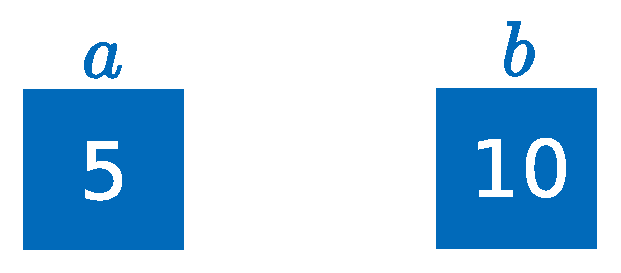
\includegraphics[scale=0.5]{figures/two_variables_example/example.eps}
        \caption{Two variables example}
    \end{figure}
\end{frame}

\begin{frame}
\frametitle{A Classic Problem with Variables (2/4)}
    In programming, a memory address (a box) can store only one value at a time
    \newline

    What happens if we put the value of $b$ in $a$? We will end up with a situation as follows:
    \begin{figure}[H]
        \centering
        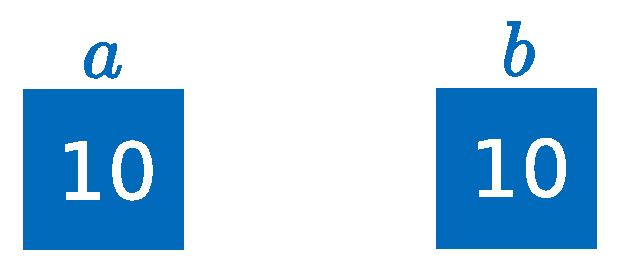
\includegraphics[scale=0.5]{figures/two_variables_example/assignment.eps}
        \caption{Two variables: $b$ assigned to $a$}
    \end{figure}
\end{frame}

\begin{frame}
\frametitle{A Classic Problem with Variables (3/4)}
    If we just assign $b$ to $a$, we will lose the value of $a$
    \newline

    How are we actually going to solve the problem of losing the value of a variable?
\end{frame}

\begin{frame}
\frametitle{A Classic Problem with Variables (4/4)}
    To solve the swapping problem, we are going to introduce a new, temporary variable
    \begin{figure}[H]
        \centering
        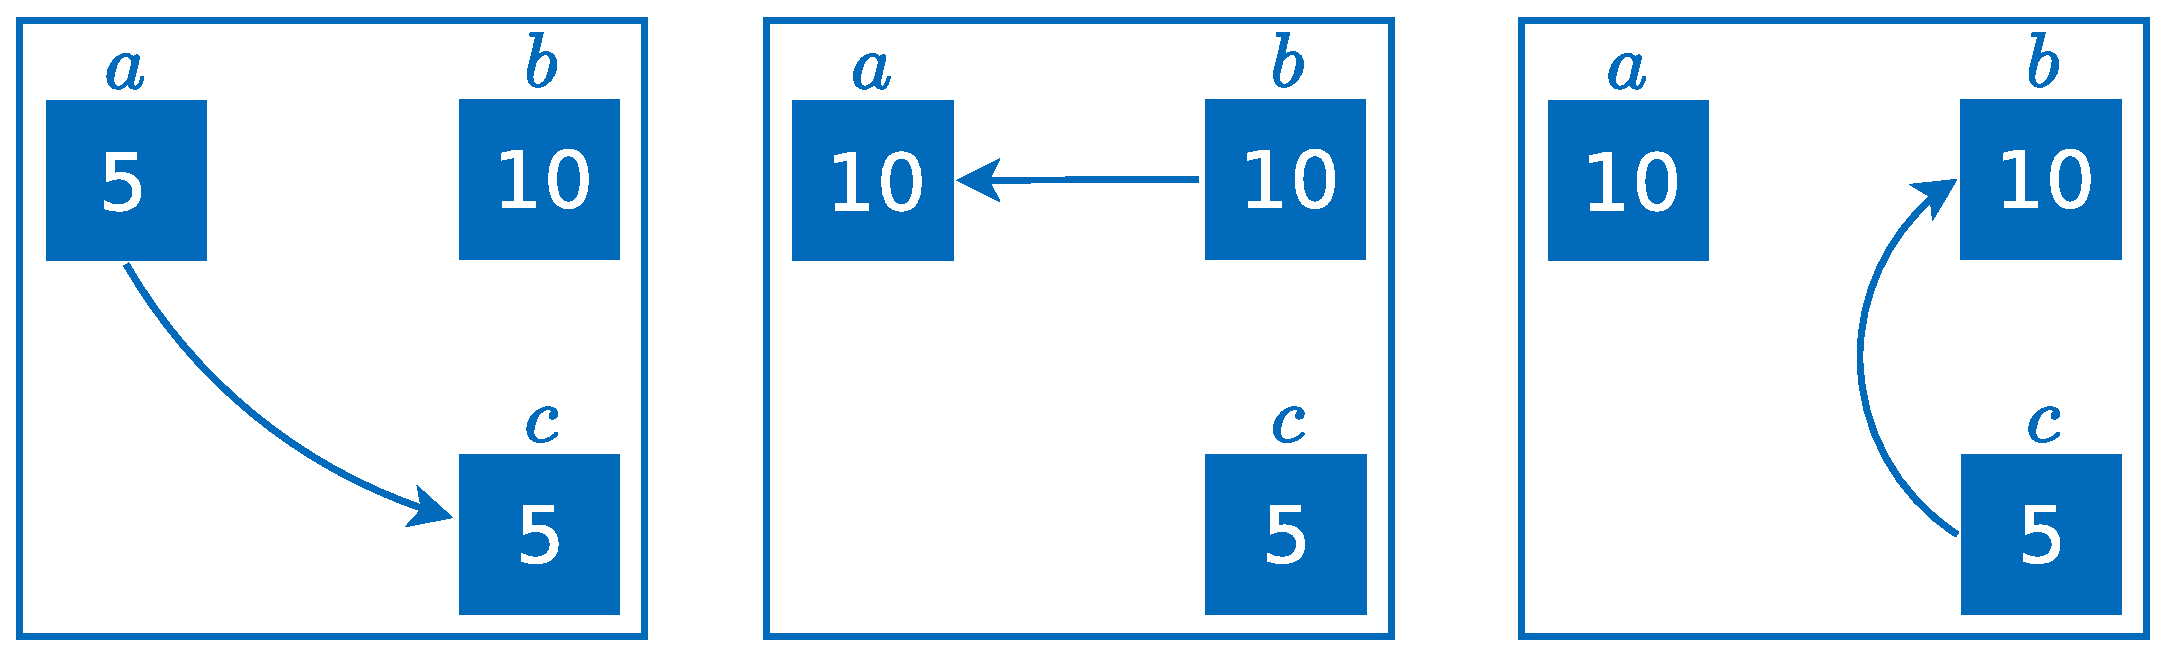
\includegraphics[scale=0.3]{figures/two_variables_example/swapping.eps}
    \end{figure}
\end{frame}

\begin{frame}
\frametitle{Variables Conclusion}
    The previous example illustrates two essential things about programming:
    \begin{itemize}
        \item The use of variables: everything we do in programming involves manipulating variables in some way
        \item The necessity for knowing what happens with the variables in your program \textbf{at any time}: if you don’t understand your program, it's \textbf{highly likely} that you will make a mistake
    \end{itemize}
\end{frame}

\section{Decisions and Loops}

\begin{frame}
\frametitle{Why Do We Need Decisions?}
    Computer programs would be useless if they could not make decisions
    \newline

    Example: suppose that you have three web browsers installed on your computer and you make browser 3 the default one. Once you do that, you expect that when you click on a link, a page will open in browser 3
    \newline

    The browser example illustrates a program that makes decisions. In this case, the operating system remembers our choice of default browser, so when we open a link, it checks
    \begin{itemize}
        \item Is browser 1 default? No
        \item Is browser 2 default? No
        \item Is browser 3 default? Yes. So open the link in browser 3
    \end{itemize}
\end{frame}

\begin{frame}
\frametitle{How Do We Program Decisions?}
    In most programming languages, the keywords for telling a program that it should do a decision at some point are \textbf{if} and its buddy \textbf{else}. If and else have the same meaning as in the English language
    \newline

    Decisions are always made by writing expressions that result in a \textbf{Boolean} value (i.e. that are either true or false)
    \vspace{0.25cm}
    \lstset{language=Python,
            basicstyle=\ttfamily\tiny,
            keywordstyle=\color{keywords},
            commentstyle=\color{comments},
            frame=lines,
            breaklines=true,
            stringstyle=\color{stringred},
            showstringspaces=false,
            identifierstyle=\color{codeblue}}
    \lstinputlisting{code_snippets/if_else_example.py}
\end{frame}

\begin{frame}
\frametitle{How Decisions Change the Flow of a Program}
    Given a program with an if and else conditions, if the value of the logical expression in the \emph{if} condition is true, the program executes only the statements in the if block
    \newline

    If the value of the logical expression in the \emph{if} condition is false, then the program proceeds by executing the statements in the \emph{else} block
    \newline

    Multiple decision branches (i.e. more than two) can be introduced by either nesting if/else blocks or using \textbf{else if} blocks (shortened to \emph{elif} in Python); these two variants are equivalent, but else if blocks make programs easier to read
\end{frame}

\begin{frame}
\frametitle{Repetitive Actions: Loops}
    Programs that perform only declarations, assignments, and decisions are not everything that we can do
    \newline

    Suppose that we want to sum 10000 numbers. Are we going to declare 10000 variables and sum them? Absolutely not; we can use \textbf{loops} for that
    \newline

    Loosely speaking, loops are actions that are performed repetitively
\end{frame}

\begin{frame}
\frametitle{Types of Loops}
    There are two types of loops in programming languages:
    \begin{itemize}
        \item \textbf{for loops}, which run a predetermined number of times (for instance, they are very useful for accessing all array elements)
        \lstset{language=Python,
                basicstyle=\ttfamily\tiny,
                keywordstyle=\color{keywords},
                commentstyle=\color{comments},
                frame=lines,
                breaklines=true,
                stringstyle=\color{stringred},
                showstringspaces=false,
                identifierstyle=\color{codeblue}}
        \lstinputlisting{code_snippets/for_loop_example.py}
        \item \textbf{while loops}, which run as long as some condition is satisfied
        \lstset{language=Python,
                basicstyle=\ttfamily\tiny,
                keywordstyle=\color{keywords},
                commentstyle=\color{comments},
                frame=lines,
                breaklines=true,
                stringstyle=\color{stringred},
                showstringspaces=false,
                identifierstyle=\color{codeblue}}
        \lstinputlisting{code_snippets/while_loop_example.py}
    \end{itemize}
\end{frame}

\begin{frame}
\frametitle{For Loops Explained}
    A for loop:
    \begin{itemize}
        \item Starts by assigning a variable (we call it a counter) and checking whether the variable is less than the maximum allowed value
        \item If it is, the statements inside the for block are executed
        \item Finally, the counter variable is incremented and the test if its value is less than the maximum allowed value is performed again
        \newline
    \end{itemize}
    Many programming languages (e.g. Python and C++ since C++11) have special types of for loops (foreach loops) that iterate over all elements of a given collections (e.g. a list)
\end{frame}

\begin{frame}
\frametitle{While Loops Explained}
    While loops generally do the same thing as for loops
    \newline

    The difference between for and while loops is that for loops run a predetermined number of times; while loops, on the other hand, can run a potentially infinite number of times
    \newline

    Note that in while loops you \textbf{must not} forget to (somehow) update the value of the variable included in the while condition; otherwise, you will run into a situation called \textbf{infinite loop}
\end{frame}

\section{Statically vs. Dynamically Typed Languages}

\begin{frame}
\frametitle{Statically and Dynamically Typed Languages}
    A statically typed language determines the type of a variable at compile time (e.g. C++, Java)
    \newline

    In dynamically typed languages, the type of a variable is determined at runtime (e.g. Python, JavaScript)
    \newline

    Dynamically typed languages are generally easier to write, but harder to debug
\end{frame}

\begin{frame}
\frametitle{Variable Types}
    The type of a variable (remember, think of it as a box) determines what the variable (the box) can store
    \newline

    In a statically-typed languages, if a variable is of type X, it can \textbf{only} store values of type X and nothing else
    \newline

    All programming languages have what we call \textbf{primitive types}; these are predefined types that we can use "off the shelf" (e.g. \emph{int}, \emph{float}, \emph{char})
\end{frame}

\begin{frame}
\frametitle{Number Types}
    Most languages have more than one type for storing numbers
    \newline

    The number types differ by the range of numbers that they can store, but also by the actual memory that they occupy
\end{frame}

\section{Compiled vs. Interpreted Languages}

\begin{frame}
\frametitle{Compilers and Interpreters (1/2)}
    Computers are binary machines (understand only 0s and 1s)
    \newline

    On the other hand, programming languages have phrases close to human languages
    \newline

    Why are the computers able to understand our programs then? Because programs are translated with the help of either compilers or interpreters
\end{frame}

\begin{frame}
\frametitle{Compilers and Interpreters (2/2)}
    Compilers "translate" a program once the program is written, i.e. when a programmer decides to compile (translate) the program (e.g. C++, Java)
    \newline

    Interpreters translate a program line by line as the program is executed (e.g. Python, JavaScript, Ruby)
\end{frame}

\begin{frame}
\frametitle{Assembly Language}
    Programs are not directly translated to machine code, but are first translated to an intermediate language, called \textbf{assembly language}
    \newline

    Assembly language is the bridge between higher level languages and low-level machine code
\end{frame}

\section{Modularity: Functions}

\begin{frame}
\frametitle{What is a Function?}
    In mathematics, a function is like a machine that takes an input and gives a specific output. Example: square root
    \begin{figure}[H]
        \centering
        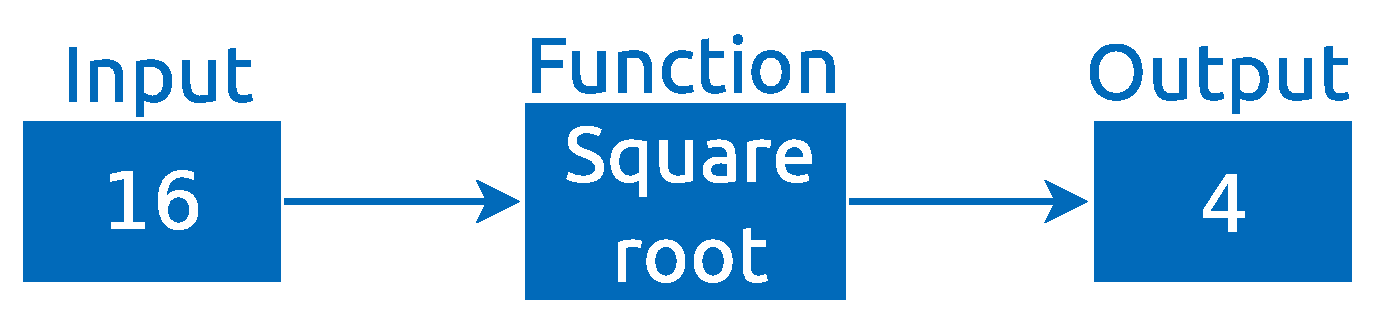
\includegraphics[scale=0.3]{figures/square_root_example.eps}
    \end{figure}
    In programming, we have two types of functions:
    \begin{itemize}
        \item Functions that do the same job as mathematical functions (i.e. return a result)
        \item Functions that do not return a result, but only perform actions
    \end{itemize}
    In languages like C++, the \textbf{void} keyword in front of the function name tells that the function does not return a value
\end{frame}

\begin{frame}
\frametitle{So, What Exactly is a Function?}
    A function is a piece of code that does a specific job and can be used with different inputs and/or in many different places in a program
    \newline

    We use functions because they allow us to separate the logic in a program; they also let us (and other programmers) reuse the code
\end{frame}

\begin{frame}
\frametitle{A Function Example (1/3)}
    Let's suppose that we want to find the maximum of two numbers
    \newline

    In principle, we could explicitly check which number is greater every time we need to do this, but our code would then be very repetitive
    \newline

    A better approach would be to define a function $max(a,b)$, which returns the larger number; we could then call this function anywhere else in our code
\end{frame}

\begin{frame}
\frametitle{A Function Example (2/3)}
    Here's a Python example of such a function (note: the $max$ function is already predefined in Python, but we define it here for illustrative purposes)
    \lstset{language=Python,
            basicstyle=\ttfamily\tiny,
            keywordstyle=\color{keywords},
            commentstyle=\color{comments},
            frame=lines,
            breaklines=true,
            stringstyle=\color{stringred},
            showstringspaces=false,
            identifierstyle=\color{codeblue}}
    \lstinputlisting{code_snippets/max.py}
    \vspace{0.5cm}

    And here's an example of how we would call the function given that we have two variables $a$ and $b$ that have the values $1$ and $2$ respectively
    \lstset{language=Python,
            basicstyle=\ttfamily\tiny,
            keywordstyle=\color{keywords},
            commentstyle=\color{comments},
            frame=lines,
            breaklines=true,
            stringstyle=\color{stringred},
            showstringspaces=false,
            identifierstyle=\color{codeblue}}
    \lstinputlisting{code_snippets/calling_max.py}
\end{frame}

\begin{frame}
\frametitle{A Function Example (2/3)}
    In our example, we used $a$ and $b$ for the variables in the main program scope, but $m$ and $n$ in our $max$ function. Why can we do that?
    \newline

    Because the function parameters are just copies of the original values. When we call $max(a,b)$, the values of $a$ and $b$ are \textbf{copied to} $m$ and $n$ respectively, so they are not actually the same variables
    \newline

    In some languages (e.g. C++), it is possible to pass a \textbf{reference} to a variable; in such case, $a$ and $m$ and also $b$ and $n$ would point to the same address in memory, but they would still be different variables
\end{frame}

\begin{frame}
\frametitle{The Function Example Visualised}
    \begin{figure}[H]
        \centering
        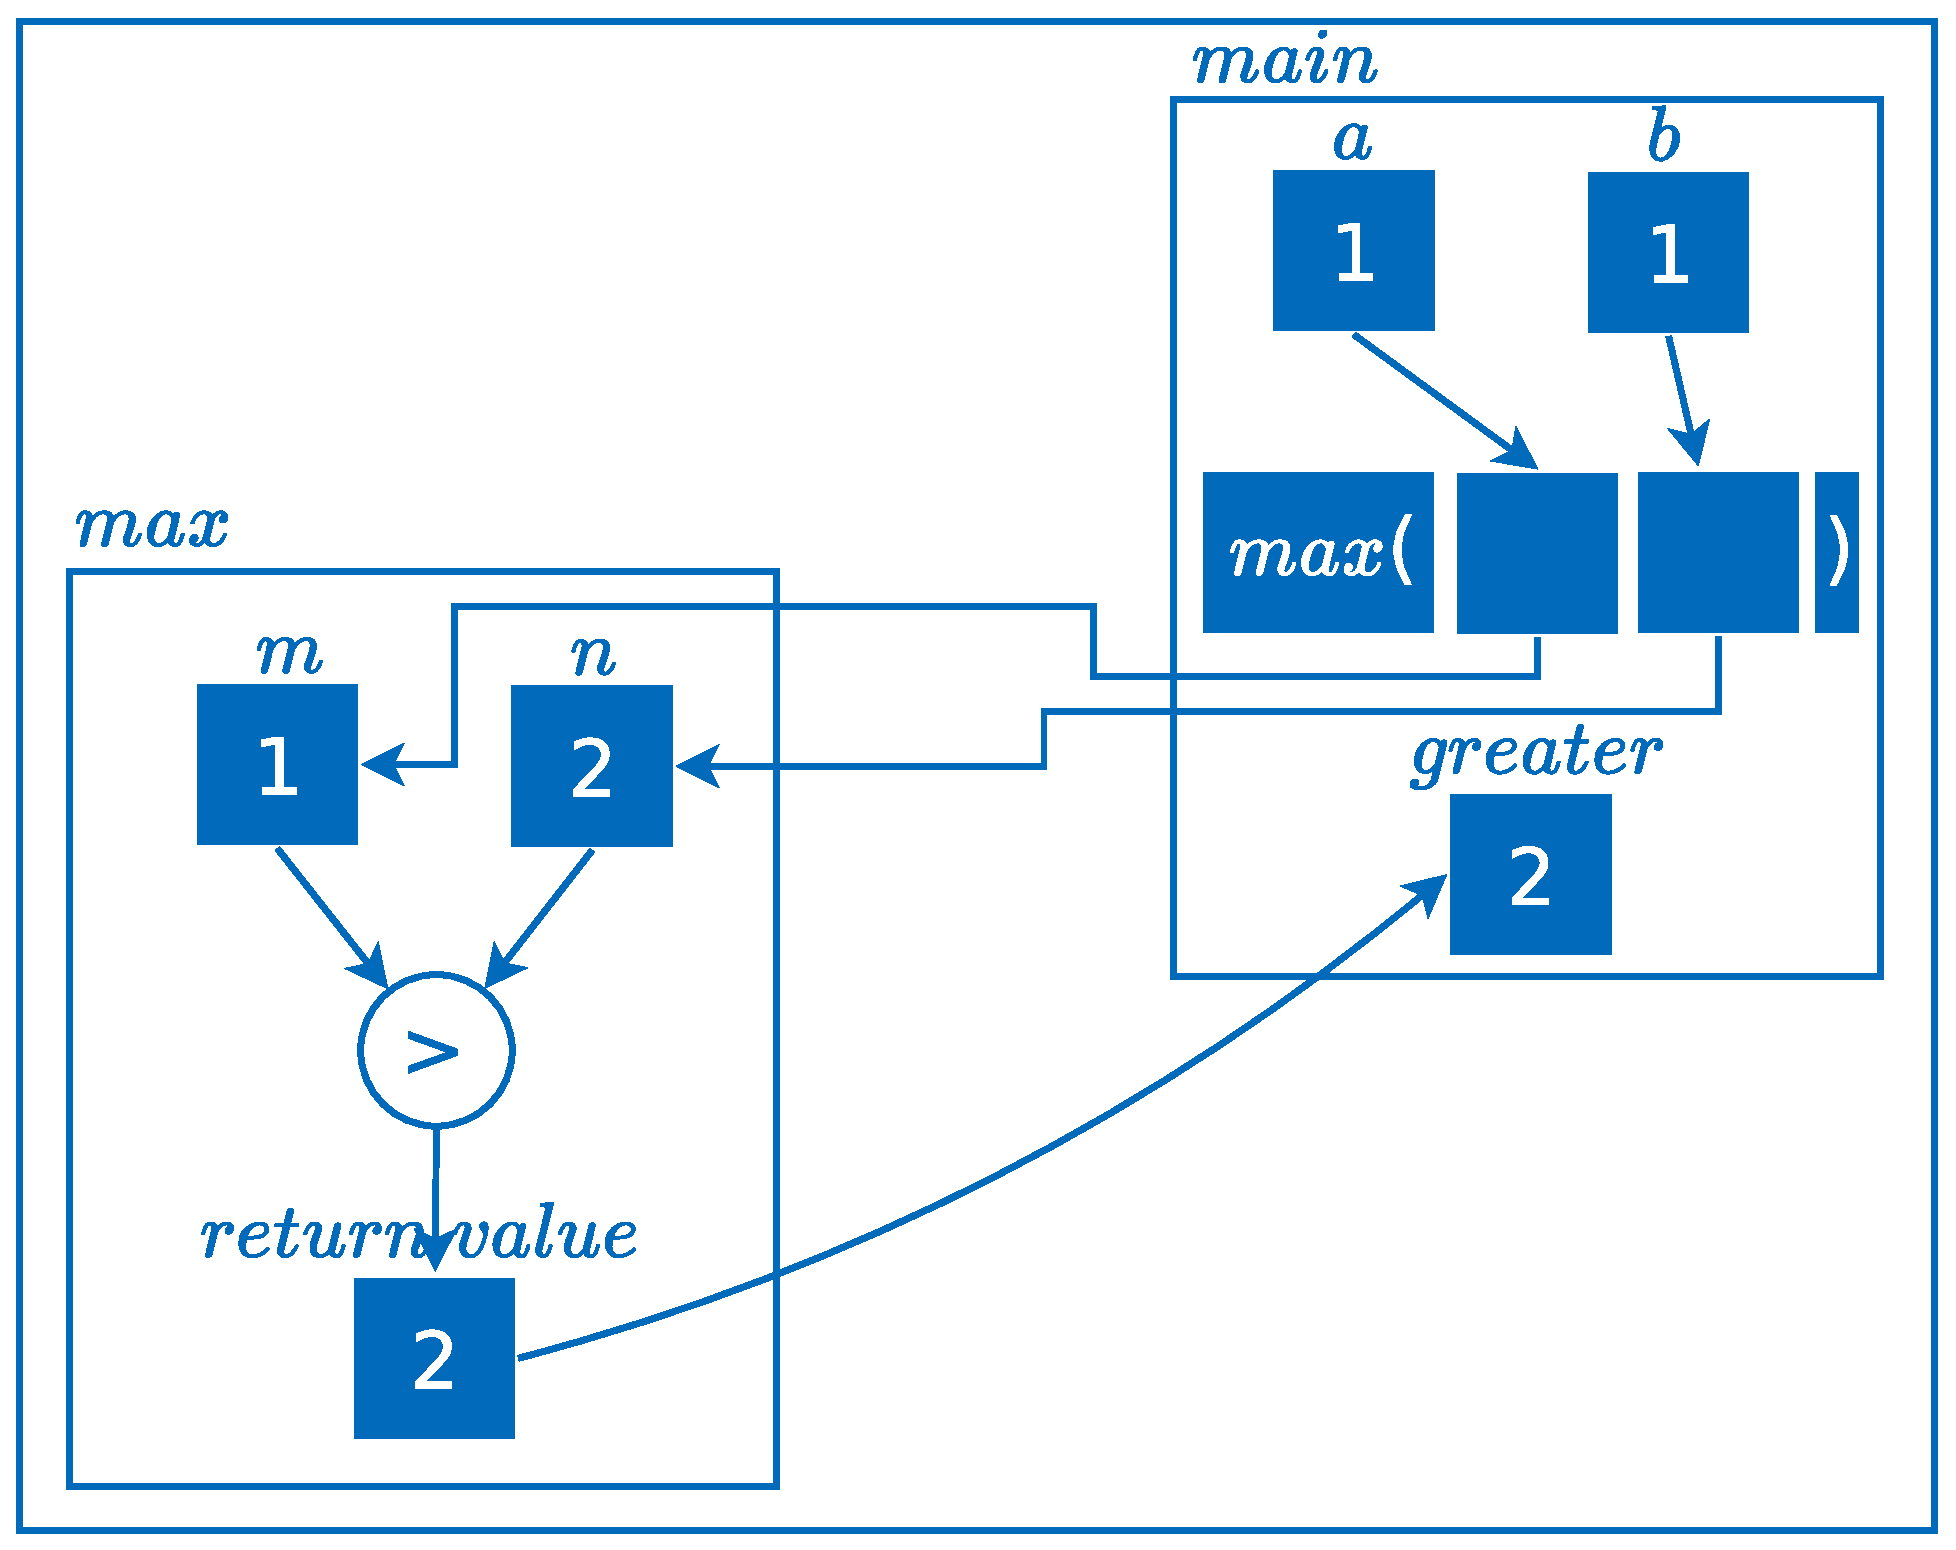
\includegraphics[scale=0.25]{figures/max_function_example.eps}
    \end{figure}
\end{frame}

\section{Programming Paradigms}

\begin{frame}
\frametitle{Imperative and Procedural Programming}
    In this slide set, we only talked about two programming paradigms:
    \begin{itemize}
        \item \textbf{imperative programming}, which is concerned with the state of a program and the commands that modify that state
        \item \textbf{procedural programming}, which heavily utilises function (procedure) calls
        \newline
    \end{itemize}

    Procedural programs are also imperative programs, but they use functions for controlling a program's state
    \newline

    These are however not the only existing programming paradigms
\end{frame}

\begin{frame}
\frametitle{Object-Oriented Programming (OOP)}
    OOP is perhaps the most common programming paradigm in even moderately complex projects
    \newline

    OOP-based programs define \textbf{classes} from which one can instantiate \textbf{objects} that have:
    \begin{itemize}
        \item \textbf{fields} that represent the objects' own internal state and
        \item \textbf{methods} that manipulate that state
    \end{itemize}

    The OOP principle of \textbf{encapsulation} allows hiding part of a program's logic from the users of a particular program module
    \newline

    Languages such as C++ and Python (both of these languages are heavily used by our research group) are not fully OOP-based, but support OOP pretty much completely; on the other hand, languages such as Java and C\# are completely OOP-based
\end{frame}

\begin{frame}
\frametitle{Logic Programming}
    Logic programming is a very different paradigm in which we represent:
    \begin{itemize}
        \item general knowledge about a certain domain as a set of logical rules
        \item specific knowledge about the domain by asserting facts
        \newline
    \end{itemize}
    A program written in a logic programming language is concerned with proving new facts from the set of known rules and facts
    \newline

    You will briefly look at one logic programming language (Prolog) in the AI course
\end{frame}

\begin{frame}
\frametitle{Functional Programming}
    Functional programming, like procedural programming, operates by using functions
    \newline

    Functions in functional programming are however closer to mathematical functions, i.e. they cannot change the state of data
    \newline

    Functional programming is more closely examined in the Master of Computer Science program; we don't do much functional programming in MAS
\end{frame}

\begin{frame}
\frametitle{}
    \begin{center}
        {\huge Thanks for your attention}
    \end{center}
\end{frame}

\end{document}
